\documentclass[border=10pt]{standalone}

\usepackage{tikz}
\usepackage{tikzsymbols}
\usetikzlibrary{calc,patterns,shapes.geometric}

\def\centerarc[#1](#2)(#3:#4:#5){\draw[#1] ($(#2)+({#5*cos(#3)},{#5*sin(#3)})$) arc (#3:#4:#5);}

\begin{document}
	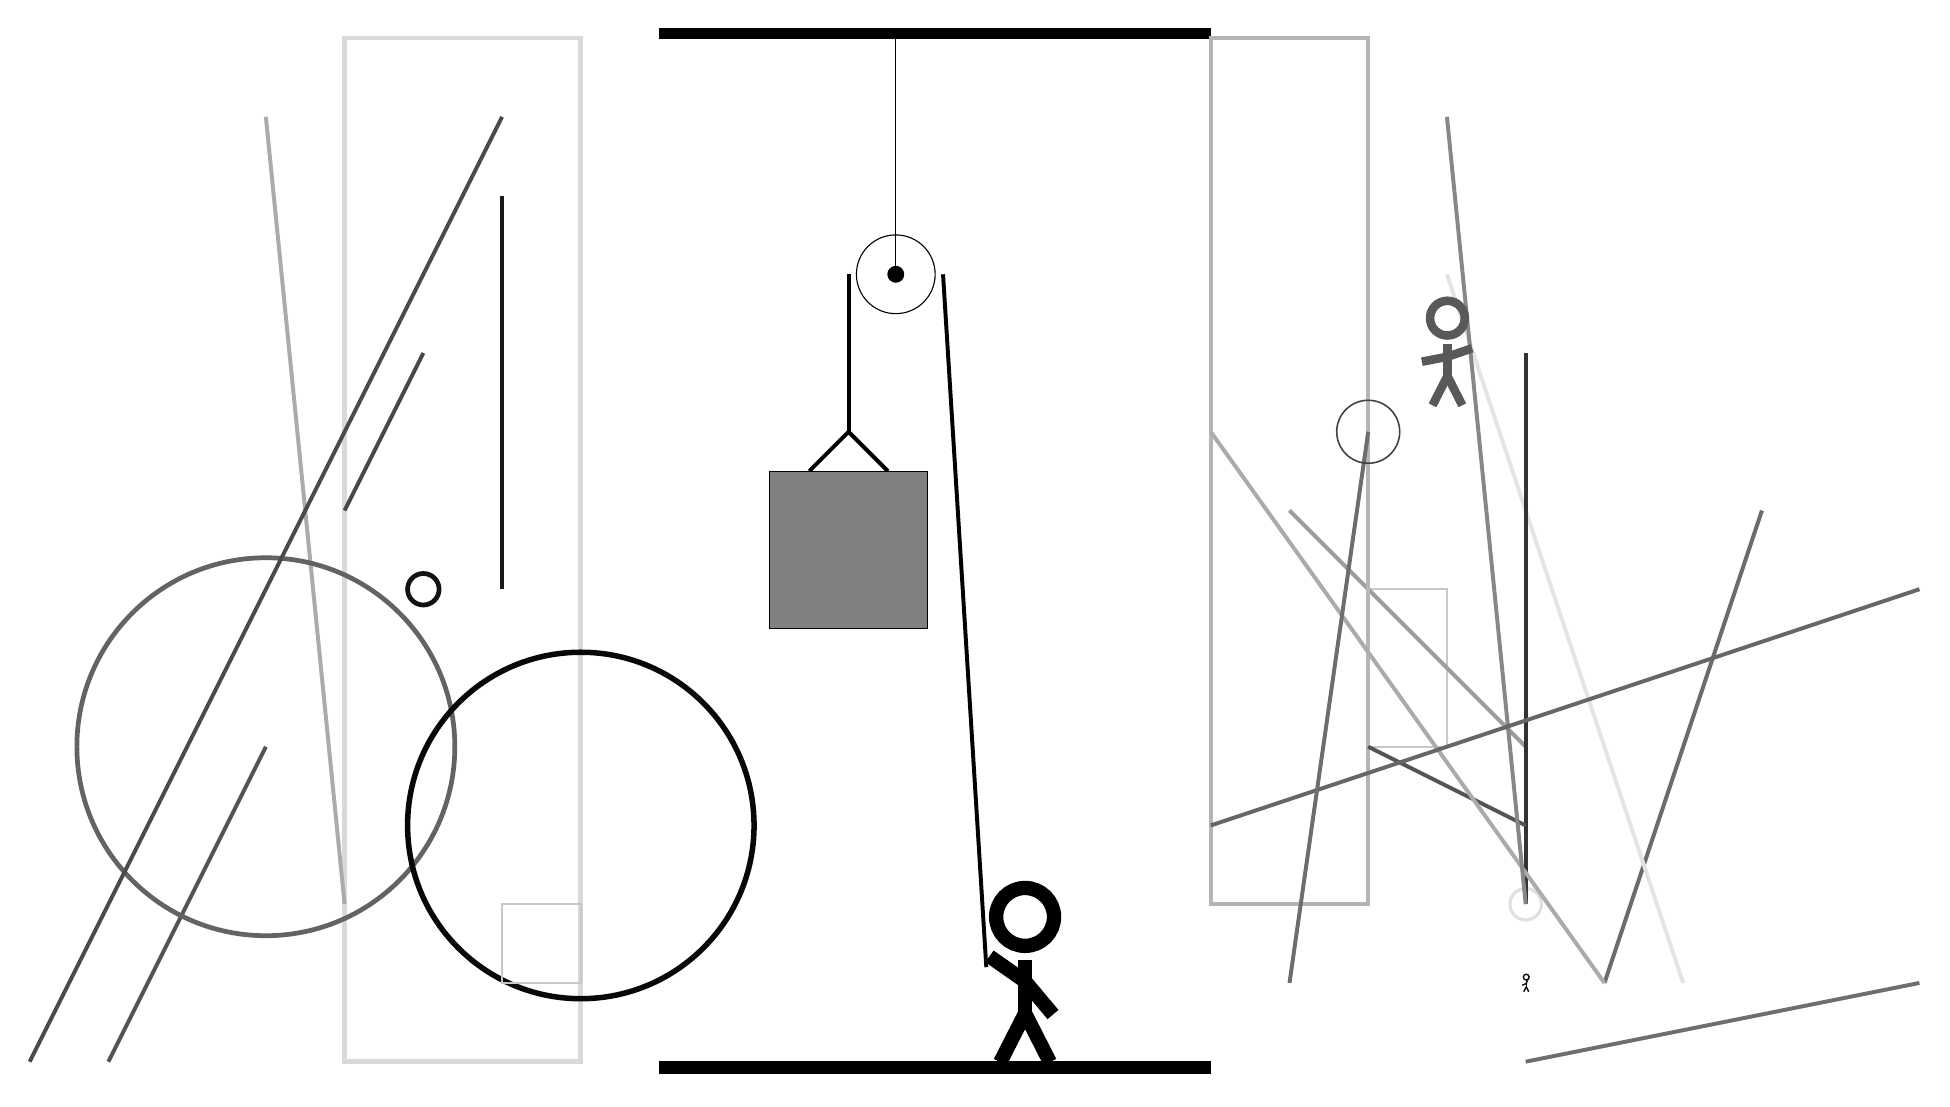
\begin{tikzpicture}
		%%%%% START %%%%%
		
		\draw[fill=black] (-2, 10) rectangle (5, 10.125);
		
		\draw (1, 7) circle (0.5);
		\draw[fill=black] (1, 7) circle (0.1);
		\draw (1, 10) -- (1, 7);
		
		\draw[line width=0.5mm] (-0.1, 4.5) -- (0.4, 5.0) -- (0.9, 4.5);
		\draw[fill=black!50] (-0.6, 4.5) rectangle (1.4, 2.5);
		
		\draw[line width=0.5mm, color=black!58](10, -2) -- (12, 4);
		
		\draw [line width=0.6mm, color=black!93](-5, 3) circle (0.2);
		\draw[line width=0.5mm, color=black!11](8, 7) -- (11, -2);
		\draw[line width=0.6mm, color=black!15] (-3, -3) rectangle (-6, 10);
		\draw[line width=0.2mm, color=black!22] (7, 3) rectangle (8, 1);
		\draw[line width=0.5mm, color=black!33](-7, 9) -- (-6, -1);
		\draw[line width=0.5mm, color=black!67](-7, 1) -- (-9, -3);
		
		\draw[line width=0.5mm, color=black!57](9, -3) -- (14, -2);
		\draw[line width=0.5mm, color=black!38](6, 4) -- (9, 1);
		
		\draw[line width=0.5mm, color=black!29] (5, -1) rectangle (7, 10);
		\draw[line width=0.5mm, color=black!72](-6, 4) -- (-5, 6);
		
		\draw [line width=0.4mm, color=black!12](9, -1) circle (0.2);
		\draw[line width=0.5mm, color=black!80](9, -1) -- (9, 6);
		
		\draw[line width=0.5mm, color=black!90](-4, 3) -- (-4, 8);
		\node[line width=0.7mm, color=black!95] at (9, -2) {\Strichmaxerl[1][23][71]};
		\draw[line width=0.5mm, color=black!67](9, 0) -- (7, 1);
		
		\draw[line width=0.5mm, color=black!33](5, 5) -- (10, -2);
		
		\draw[line width=0.5mm, color=black!47](9, -1) -- (8, 9);
		\draw [line width=0.6mm, color=black!61](-7, 1) circle (2.4);
		\draw[line width=0.5mm, color=black!60](5, 0) -- (14, 3);
		\draw[line width=0.5mm, color=black!57](6, -2) -- (7, 5);
		\node[line width=0.3mm, color=black!65] at (8, 6) {\Strichmaxerl[6][11][19]};
		
		\draw [line width=0.7mm, color=black!97](-3, 0) circle (2.2);
		\draw[line width=0.5mm, color=black!71](-4, 9) -- (-10, -3);
		\draw[line width=0.2mm, color=black!22] (-4, -2) rectangle (-3, -1);
		
		\draw [line width=0.2mm, color=black!75](7, 5) circle (0.4);
		
		\draw[line width=0.5mm] (0.4, 7) -- (0.4, 5.0);
		\centerarc[line width=0.5mm](1, 7)(0:180:0.6);
		\draw[line width=0.5mm](1.6, 7) -- (2.15, -1.8);
		
		\node at (2.6, -1.9) {\Strichmaxerl[10][-35][-50]};
		
		\draw[fill=black] (-2, -3) rectangle (5, -3.15);
		
		%%%%% END %%%%%
	\end{tikzpicture}
\end{document}